\chapter{Projektkontext}

\section{Das Projekt Charigame}

Das Projekt Charigame entstand ursprünglich als interne Initiative der elancer-team GmbH mit dem Ziel eine digitale Spendenaktion zu ermöglichen.
Diese Idee des Projekts lässt sich auf eine durch die Agentur erstellte Weihnachtsaktion zurückführen, die auf der Website \texttt{https://hohoho.elancer-team.de/} implementiert wurde.
Bei der Spendenaktion hat die elancer-team GmbH die Spendensumme bereitgestellt und die Agenturkunden wurden eingeladen teilzunehmen und durch ihr engagement den Spendentopf zu erhöhen.
Diese Plattform ermöglichte es den Kunden der Agentur erstmals, über die gamifizierte Benutzeroberfläche Spenden zu erspielen und zu verteilen.
\\\\
Die positive Resonanz der Agenturkunden auf diesen gamifizierten Ansatz führte zu der Überlegung das Konzept weiterzuentwickeln.
Aufgrund der erfolgreichen Durchführung äußerte ein Kunde der Agentur den Wunsch, eine vergleichbare Spendenaktion für das eigene Unternehmen zu realisieren.

Diese erste kundenspezifische Umsetzung basierte auf einer abgewandelten Kopie der Weihnachts-Spendenaktion.
Die Anfrage stellte dann den Übergang von einem internen Projekt zu einem eigenständigen Dienstleistungsangebot dar.
Daraufhin wurde durch den Autor das Projekt Charigame als eigenständiges Wordpress-Plugin realisiert.
Das daraus resultierende Wordpress-Plugin befindet sich aktuell bei einem Kunden im produktiven Einsatz und bildet die Grundlage für die in dieser Arbeit dokumentierten technischen Analyse und Weiterentwicklung.
\\\\
\textbf{Funktionsweise von Charigame}
\\\\
Die Funktionsweise von Charigame lässt sich grob in 5 Schritte unterteilen, die in Abbildung~\ref{fig:charigame-funktion}: veranschaulicht sind:

%\begin{figure}[!ht]
%    \centerline{\includesvg[width=1\columnwidth]{images/firstPartyCookie.svg}}
%    \caption{Entstehungsprozess von First Party Cookies}
%\end{figure}
\begin{figure}[tbh]
    \centering
    \includesvg[width=0.88\textwidth]{images/funktionsweise_charigame}
    \caption{Funktionsweise Charigame}
    \label{fig:charigame-funktion}
\end{figure}
\newpage

\begin{enumerate}
    \item \textbf{Aufbau der Kampagne und Mailing}
    \\ Eine Spendenkampagne wird im Backend von Charigame angelegt.
    Anschließend werden Personendaten der Kunden in das System importiert.
    Das System versendet dann, basierend auf den Kampagneneinstellungen, automatisierte E-Mails mit dem Link zur Spendenaktion.
    \item \textbf{Kundeninteraktion und Spendenspiel}
    \\ Der Kunde öffnet den personalisierten Code in der E-Mail oder gibt den darin enthaltenen Code auf der Login-Page ein.
    Die in der Kampagne eingestellte Charigame-Landingpage wird angezeigt und der Kunde kann aktiv beim Spendenspiel teilnehmen.
    \item \textbf{Spielende und Spendenverteilung}
    \\ Nachdem das Spendenspiel seitens des Kunden absolviert wurde, kann dieser den erspielten Beitrag prozentual auf einen von bis zu drei verschiedenen Spendenempfängern verteilen.
    \item \textbf{Dankesseite}
    \\ Eine Dankesseite wird angezeigt und der Kunde kann nach Belieben erneut an dem Spiel teilnehmen, um seine Punktzahl zu verbessern.
    Ferner werden weitere Handlungsauforderungen in Form von CTAs ausgespielt, die den Kunden gezielt auf Bereiche des Unternehmens leiten können.
\end{enumerate}

\section{Deskriptiver Stand}
\subsection{Darstellung und Einstellungen im Wordpress Front- und Backend}
Der deskriptive Stand von Charigame befindet sich in einem funktionsfähigen, jedoch technisch und konzeptionell ausbaufähigen Zustand.
Das Wordpress-Plugin integriert sich in das CMS Wordpress und erweitert den Funktionsumfang, um gamifizierte Spendenaktionen.
Bevor die Spendenaktion bereitsteht ist es notwendig, dass verschiedene Einstellungen getroffen.
Die notwendigen Einstellungen können über das Wordpress-Backend Menü aufgerufen werden.
\\
Hierzu erzeugt ein Charigame Menüpunkt im Wordpress Dashboard wie in Abbildung~\ref{fig:charigame-menu-legacy}: visualisiert.
In diesem Menü sind die wichtigsten Einstellmöglichkeiten als Menüpunkte definiert.
\begin{figure}[tbh]
    \centering
    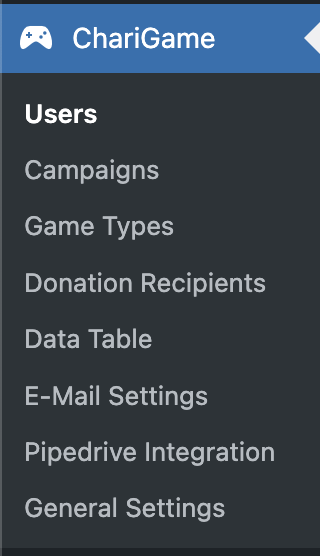
\includegraphics[width=0.2\textwidth]{images/legacy_charigame_wordpress_menu}
    \caption{Charigame Menü im Wordpress Dashboard}
    \label{fig:charigame-menu-legacy}
\end{figure}

Die im Menü angezeigten Einstellungen und Informationen lassen sich in mehrere Kategorien gliedern.
Diese spiegeln den Aufbau der einzelnen Bausteine vom Projekt wider und werden nachfolgend erläutert.
\\\\
\textbf{General Settings}\\\\
Die General Settings enthalten grundlegende Angaben zum Unternehmen, das eine Spendenkampagne durchführt.
Neben rechtlichen Informationen wie dem Impressum und der AGBs können hier auch gestalterische Parameter wie Farben der Corporate Identity hinterlegt werden.
Die Backendansicht der Einstellungsseite ist in Abbildung~\ref{fig:charigame-general-settings-legacy} dargestellt.
\begin{figure}[H]
    \centering
    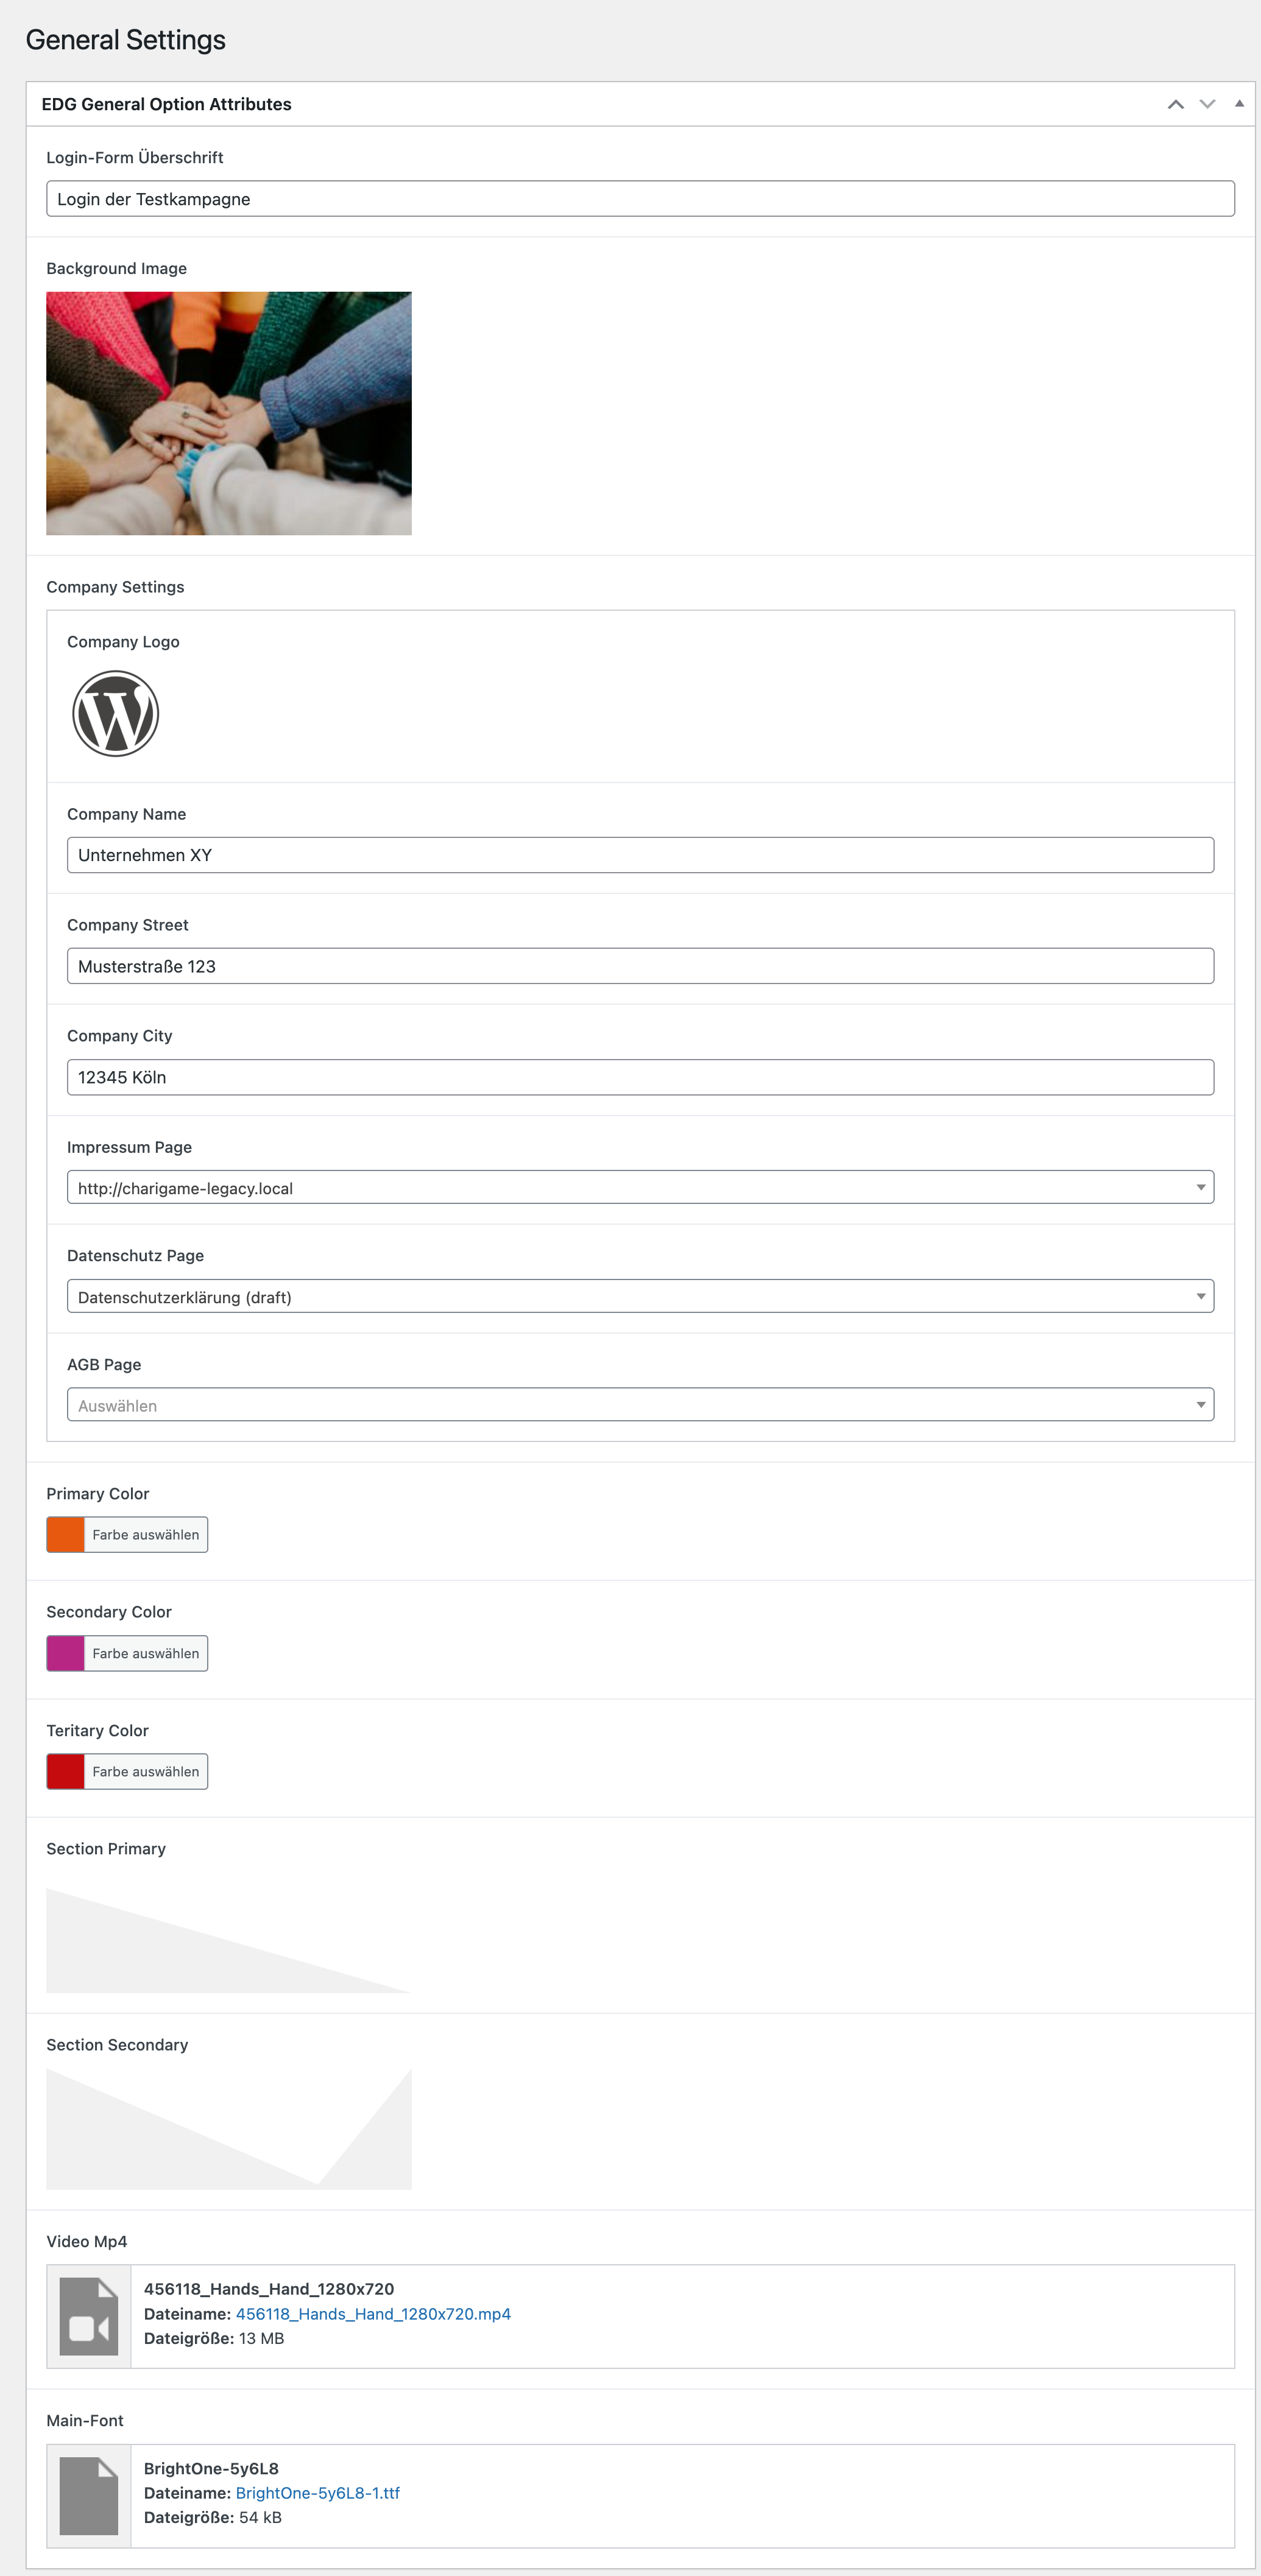
\includegraphics[width=0.7\textwidth]{images/legacy_general_settings}
    \caption{General Settings im WordPress Backend}
    \label{fig:charigame-general-settings-legacy}
\end{figure}

Im Detail können grundlegende Einstellungen konfiguriert werden, z.B.:
\begin{itemize}
\item Überschriften der Login-Form
\item Hintergrund- und Logo-Uploads
\item Farbschema (Primär, Sekundär, Teritär)
\end{itemize}
Eine vollständige Übersicht der Eingabefelder ist im Anhang zu finden (vgl. Tabelle~\ref{tab:eingabefelder_general_settings}).
\\\\
Die getroffenen Einstellungen bestimmen direkt das Erscheinungsbild der Login-Form im Frontend (vgl. Abbildung~\ref{fig:login-textkampagne}).

\begin{figure}[H]
    \centering
    
\includegraphics[width=0.8\textwidth]{images/legacy_login_testkampagne}
    \caption{Login-Form einer Charigame-Testkampagne im Frontend}
    \label{fig:login-textkampagne}
\end{figure}

\textbf{Donation Recipients}\\\\
Die Donation Recipients stellen die Empfänger der Spenden dar.
Für jede Kampagne müssen mindestens drei Empfänger angelegt werden.
Pro Empfänger werden ein Name, ein Bild sowie ein beschreibender Text hinterlegt (vgl. Tabelle~\ref{tab:eingabefelder_donation_recipients}).
Das vorab erstellen der Recipients ist im Verlauf der Einstellungen zwingend erforderlich, da sie in den Kampagneneinstellungen referenziert werden.
Die Backendansicht der Donation Recipients ist in Abbildung~\ref{fig:donation-recipients-settings-legacy} veranschaulicht.
\begin{figure}[H]
    \centering
    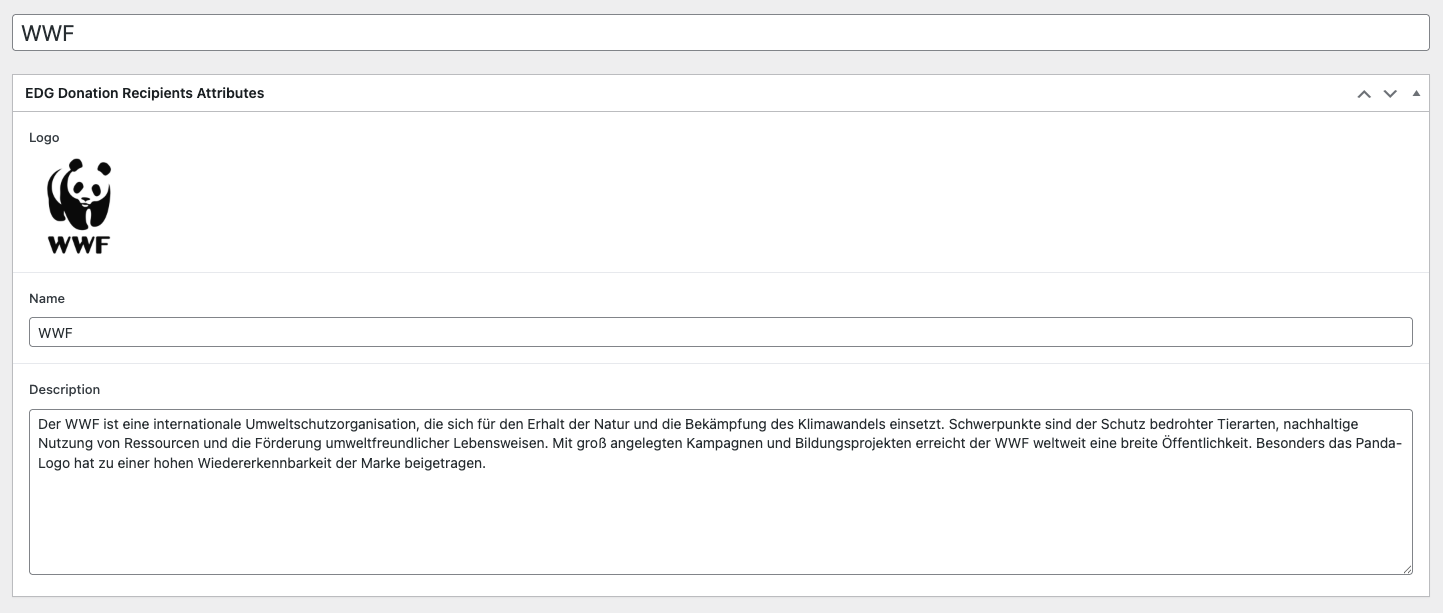
\includegraphics[width=1\textwidth]{images/legacy_donation_recipients_backend}
    \caption{Donation Recipients im WordPress Backend}
    \label{fig:donation-recipients-settings-legacy}
\end{figure}
Die im Backend gesetzten Einstellungen werden in folgender Form wie (vgl. Abbildung~\ref{fig:donation-recipients-frontend-legacy}) im Frontend dargestellt:
\begin{figure}[H]
    \centering
    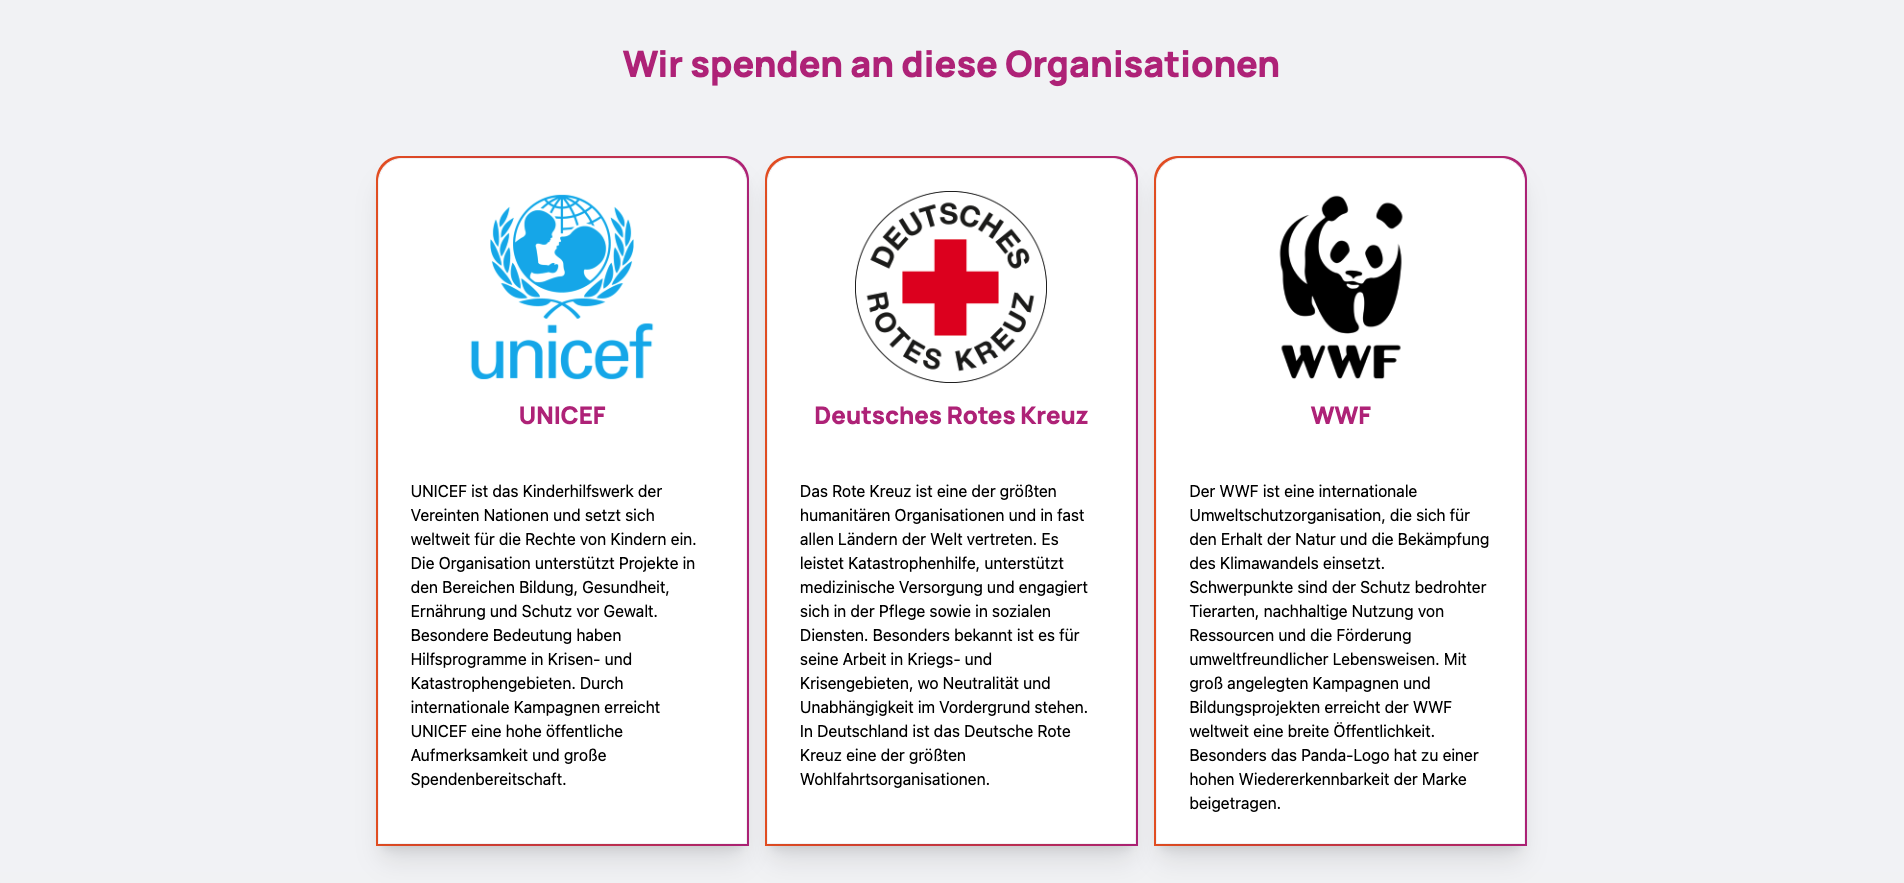
\includegraphics[width=1\textwidth]{images/legacy_donation_recipients_frontend}
    \caption{Donation Recipients im WordPress Frontend}
    \label{fig:donation-recipients-frontend-legacy}
\end{figure}

\newpage
\textbf{Game Types}\\\\
Unter Game Types werden die verfügbaren Spieltypen definiert.
Jedes Spiel kann vom Unternehmen mit einer \glqq How-To-Play\grqq{}-Anleitung versehen werden.
Diese besteht aus einer Abfolge von Schritten, die jeweils mit einem Icon, einer Überschrift und einem erklärenden Text ergänzt werden können.

Bild Backendansicht -- Bild Frontendansicht

\\\\
\textbf{Users \& Pipedrive Integration}\\\\
Im Menüpunkt Users können die Teilnehmer der Spendenkampagnen verwaltet werden.
Für ein Kundenprojekt wurde zudem eine Pipedrive-Integration entwickelt, welche über die \gls{REST}-\gls{API} automatisch Kontaktdaten aus dem CRM-System importiert.
\begin{itemize}
    \item Vorname
    \item Nachname
    \item Geburtsdatum
    \item E-Mail-Adresse
    \item Flags: Imported, E-Mail sent
\end{itemize}

Bild Backendansicht


\\\\
\textbf{E-Mail-Settings}\\\\
Das Plugin erlaubt es, anstelle des standardmäßigen WordPress-Mailers einen eigenen SMTP-Server einzubinden.
Dafür stehen folgende Eingabefelder bereit:
\begin{itemize}
    \item SMTP-Host
    \item SMTP-Port
    \item Benutzername
    \item Absender-E-Mail
    \item Absender-Name
\end{itemize}
Aus Sicherheitsgründen kann das Passwort optional in der wp-config.php als Konstante hinterlegt werden, sodass es nicht in der Datenbank gespeichert wird.
Zusätzlich bietet die Oberfläche eine Funktion zum Versand einer Testmail, mit der sich die Konfiguration überprüfen lässt.

Darüber hinaus bietet der Backend-View der E-Mail-Settings eine kleine Funktion, eine Testmail an eine ausgewählte Adresse zu senden um die Einstellungen auf Ihre richtigkeit prüfen zu können.

\\\\
\textbf{Data Table}\\\\
Die Data Table dient als zentrales Dashboard, um die Ergebnisse und Kennzahlen der Spendenkampagnen auf einen Blick darzustellen.
Angezeigt werden u. a.:
\begin{itemize}
    \item erstellte Kampagnen
    \item zugehörige Spendenempfänger
    \item Benutzername
    \item aktueller Spendenstand (in Euro)
    \item Nutzerübersicht mit einzigartigen Game Codes
\end{itemize}
Darüber hinaus werden weitere Metriken bereitgestellt, darunter Valid From, Valid Until, Last Played, Highscore, Recipient 1–3 sowie E-Mail sent.
Die genaue Bedeutung dieser Kennzahlen ist in Tabelle XY im Anhang erläutert.

%TODO: Umschreiben! Campaings einmal komplett und die oberen Punkte ebenfalls
\\\\
\textbf{Campaigns}\\\\
\\\\\\
Die Campaigns stellen das zentrale Element von Charigame dar und repräsentieren den konzeptionell und technisch komplexesten Bereich des Plugins. Dieses Modul führt sämtliche relevanten Informationen einer Spendenkampagne zusammen und ermöglicht deren Steuerung über umfangreiche Konfigurationsmöglichkeiten. Der gesamte Ablauf einer Kampagne kann somit innerhalb des WordPress-Backends abgebildet werden. Dies umfasst sowohl die Auswahl des Spielmechanismus als auch die Kommunikation mit den Teilnehmenden.

Zu den wesentlichen Komponenten gehören:

\begin{itemize}
\item \textbf{Allgemeine Kampagneninformationen} \
Jede Kampagne erhält einen Titel, eine kurze Bezeichnung sowie eine ausführliche Beschreibung. Diese Inhalte bilden die Grundlage für die Frontend-Darstellung und dienen der inhaltlichen Rahmung der Aktion. Ergänzende Medien wie Logos oder Illustrationen können hochgeladen und der Kampagne zugeordnet werden.
\item \textbf{Spielmechanik} \\
Der gewünschte Spieltyp wird aus den im System verfügbaren \textit{Game Types} ausgewählt. Dadurch wird die konkrete Mechanik der Spendenaktion definiert. Begleitende Hinweise, beispielsweise eine How-to-Play-Anleitung, können zusätzlich hinterlegt werden.

\item \textbf{Spendenempfänger (Recipients)} \\
Jede Kampagne bindet mindestens drei zuvor definierte \textit{Donation Recipients} ein. Diese Empfänger werden im Spiel zur Auswahl gestellt und gewährleisten die ordnungsgemäße Verteilung der generierten Spenden auf die vorgesehenen Organisationen.

\item \textbf{Punkte- und Spendenlogik} \\
Die Verknüpfung von Spielergebnissen mit der Spendenhöhe bildet ein zentrales Element. Über eine Highscore-Logik wird festgelegt, wie viele Punkte maximal erreichbar sind und welche Spendenwerte daraus resultieren. Gewinnkategorien ermöglichen eine Staffelung nach erreichten Punktzahlen (beispielsweise ab 20 Punkten 4 Euro, ab 50 Punkten 10 Euro). Dadurch entsteht ein direkter Zusammenhang zwischen Spielerfolg und Spendenbetrag. Ein übergeordnetes Spendenziel in Euro kann den Gesamtumfang der Kampagne begrenzen und als Fortschrittsindikator fungieren.

\item \textbf{Zeitliche Steuerung} \\
Kampagnen können zeitlich präzise geplant werden. Start- und Enddatum bestimmen den Gültigkeitszeitraum. E-Mails lassen sich automatisiert zu definierten Terminen versenden, um Teilnehmer gezielt zu aktivieren oder zu informieren.

\item \textbf{Kommunikation (E-Mail und Social Media)} \\
Für jede Kampagne können individuelle E-Mail-Texte konfiguriert werden. Diese umfassen Betreffzeile, Header, Haupttext sowie Signatur. Die Nachrichten informieren Nutzer über ihre Teilnahme, bedanken sich oder liefern Hintergrundinformationen zur Aktion. Optional kann ein E-Mail-Template mit HTML-Header und Footer gestaltet werden. Social-Media-Kanäle können durch die Hinterlegung von Links und Icons eingebunden werden, um die Reichweite der Kampagne zu erhöhen.

\item \textbf{Call-to-Action (CTA)} \\
Eine gezielte Weiterleitung kann eingerichtet werden. Hierzu werden Headline, Beschreibungstext, Button-Beschriftung und Ziel-URL definiert. Der CTA motiviert Teilnehmende nach Abschluss des Spiels oder nach Erhalt einer E-Mail zu weiteren Aktionen, beispielsweise dem Besuch einer Unternehmensseite oder einer weiterführenden Spendenkampagne.
\end{itemize}

Das Campaign-Modul ermöglicht nicht nur die inhaltliche und technische Konfiguration einzelner Kampagnen, sondern vereint auch die Schnittstellen zu Spendenlogik, Kommunikation und externer Reichweitensteigerung. Es bildet somit die Schaltzentrale von Charigame, in der organisatorische, spielmechanische und kommunikative Elemente in einer konsistenten Benutzeroberfläche zusammengeführt werden.

GSAP als Animation
Confetti JS Animation
NPM Pakage Manager
Tailwind CSS

Anhang
Login Page --
Gesamte Landingapge --
Dankesseite --

\subsection{Architektur}
So und dann auf Architektur eingehen.
CPTs nice
nur eine zentrale Plugin Datei
Screenshots Frontend Backend zeigen
Abhängigkeit ACF Pro generell acf als weiteres plugin

Bearbeitung von LP nur sehr eingeschränkt möglich viele texte statisch hinterlegt
Dashboard sehr Rudimentär und keine guten KPIs oder einblicke gesxhweige denn gutes visual design sehr einfach
Security keinen tiefergehenden augenmerk ?? Das vllt sogar außen vor lassen man munkelt....
https://natuerlich.reisen/wp-admin/post.php?post=999998&action=edit -- code ist nicht einzigartig
\section{Stakeholder und Nutzungskontext}
Als Stakeholder wurden seitens der elancer-team GmbH die folgenden Gruppen identifiziert:
Viereck mit den Stakeholdern.

Nutzungskontext: Für

\section{Gesetzte Anforderungen an die Weiterentwicklung}

Für den zu bearbeitenden Part im Kaptiel 4 sind Praxispart mindestens die folgenden Anforderungen gesetzt:
\subsection{Technische Anforderungen}
\begin{itemize}
    \item Das System muss die Abhängigkeit von der PRO-Version des Plugins ACF (Advanced Custom Fields) entfernen.
    \item Das System muss gängige WordPress-Plugin-Best-Practices befolgen.
    \item Das System soll gängige Security-Best-Practices der WordPress-Developer-Ressourcen berücksichtigen.
\end{itemize}



\subsection{Funktionale Anforderungen}
\begin{itemize}
    \item Das System muss die Landingpage mit dem Gutenberg-Editor editierbar machen.
    \item Das System muss Blöcke bereitstellen, die die bestehende Landingpage abbilden können.
    \item Das System soll eine verbesserte Version des Dashboards bereitstellen.
    \item Das System soll eine bessere Übersicht für Nutzer:innen bieten.
    \item Das System soll eine verbesserte Möglichkeit bieten, die Front-End Views (z. B. E-Mail-Templates) zu stylen.
\end{itemize}

\section{Abgrenzung des Projektumfangs}
Zur Abgrenzung des Projektumfangs wurden jetzt hier die Anforderungen aufgebaut.
Ferner gilt es begleitend die schriftliche Ausarbetiung auszuführen.
Damit ein wissenschaftlicher konsens gefunden werden kann muss das ergebnis am ende evaluiert werden und das ergebnis kritisch betrachtet werden.
Ferner soll der weitere horizont für das zukünfitge vorgehen festgelegt werden und mögliche erweiterungen oder anpassungen angesprochen werden.
